\chapter{Miscelaneous} \label{chp:misc}
\epigraph{Real stupidity beats artificial intelligence every time.}{Terry Pratchett}

An diesem Punkt haben wir bereits die wichtigsten Elemente der Sprache kennen gelernt. Hier möchte ich Ihnen noch einige nützliche Ding zeigen, die für sich keine geschlossene Einheit mehr bilden, bevor wir in den letzten beiden Kapiteln interessante Anwendungen der erlernten Techniken betrachten werden.

\section{Zeitpunkte}
Für einen Menschen ist ein Zeitpunkt gegeben durch sechs Zahlen: Jahr, Monat, Tag, Stunde, Minute und Sekunde. Diese Unterteilung ist im Alltag zwar nützlich, macht das Rechnen mit Zeitpunkten aber kompliziert. Wie viele Sekunden lagen zwischen 2019-06-21, 20:26:35 (dem Zeitpunkt, an dem diese Zeile geschrieben wurde) und 1989-03-29, 00:03:15 (dem Geburtstag des Autors)? Der Header \texttt{<time.h>} definiert Funktionen, die bei solchen Aufgaben hilfreich sind. Lesen Sie hierzu im Detail unter den Links von \url{https://en.cppreference.com/w/c/chrono}.

\subsection{UNIX Epoch Time}
Es ist leichter, mit zwei Zahlen zu rechnen, als mit zwölf\footnote{Citation needed}. Daher werden Zeitpunkte intern für den Rechner auf eine einzige Zahl herunter gebrochen: Die Zahl der Sekunden, die seit 1970-01-01, 00:00:00 vergangen sind. Dieser genormte Zeitpunkt wird \emph{UNIX Epoch Time} oder auch \emph{die UNIX-Epoche} genannt. Kennt man diese Zeitdifferenz, so kann man die Zeit zwischen zwei Punkten einfach als Differenz berechnen. Natürlich bedeutet es einen gewissen Aufwand, diese Differenz wieder in ein menschenlesbares Format zu bringen; hierzu stehen aber Funktionen bereit, die die komplizierteren Schritte (Einbeziehen von Schaltjahren, Schaltsekunden, Zeitzonen, ...) übernehmen.

Der C-Standard definiert den Datentyp \mintinline{c}{time_t} für die Arbeit mit Zeitpunkten. Das bedeutet insbesondere, dass die Funktionen, die Sie hier kennen lernen werden, Argumente vom Typ 
\mintinline{c}{time_t} annehmen werden. Die Definition von \mintinline{c}{time_t} legt jedoch nur Eigenschaften fest, nicht, wie der Datentyp exakt umgesetzt werden soll. Üblicherweise (und insbesondere beim \texttt{gcc}) handelt es sich um einen Alias für einen \mintinline{c}{long long int}, also eine \emph{vorzeichenbehaftete} 64bit-Ganzzahl. Auf älteren Systemen kann der Typ aber auch zu einem \mintinline{c}{long int}, also einer 32bit-Ganzzahl umgesetzt werden. 

Beide Zahlentypen können nur Werte einer bestimmten Größe speichern, \ie es gibt einen spätesten Zeitpunkt, den unixoide Systeme verarbeiten können. Für 64bit-Werte liegt dies in der fernen Zukunft\footnote{Genauer: am vierten Dezember des Jahres 292\,277\,026\,596. Quelle: \url{https://ximalas.info/2015/03/10/when-does-the-64-bit-unix-time_t-really-end/}}, aber bei 32bit wäre keine Zeit nach 2038-01-19, 03:14:07 darstellbar. Eine neue Epoche zu definieren wirft Kompatibilitäsprobleme auf -- woraus soll ein Programm ermitteln, auf welche Epoche sich ein Zeitwert bezieht? Für IT-Spezialisten war dieses \emph{Jahr 2038-Problem} lange Zeit ein großes Problem, bis es durch die flächendeckende Einführung von 64bit-Rechnern umgangen werden konnte.

\begin{figure}
\begin{center}
	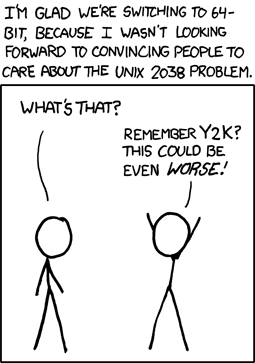
\includegraphics[width=.3\linewidth]{./gfx/xkcd-2038}
	\caption
	[Das \emph{Jahr 2038-Problem}]
	{Das \emph{Jahr 2038-Problem}. Quelle: \url{https://xkcd.com/607/}}
\end{center}
\end{figure}

\subsection{Zeitwerte finden und umrechnen}
Die aktuelle UNIX-Zeit wird von der Funktion \texttt{time} ermittelt. Dieser kann ein Pointer auf ein Objekt vom Typ \mintinline{c}{time_t} übergeben werden, an den die aktuelle Zeit (also die Zahl der Sekunden seit 1970-01-01, 00:00:00) geschrieben werden soll. Alternativ ist auch der Wert \texttt{NULL} als Parameter zulässig -- dann wird kein Wert in den Speicher geschrieben. In beiden Fällen enthält der Rückgabewert die Information der UNIX-Zeit.

\begin{codebox}[Beispiel: \texttt{time}]
\begin{minted}[linenos]{c}
#include <stdio.h>
#include <time.h>

int main () {
  time_t now = time(NULL);
  
  // time(&now);  // alternative Methode
  
  printf("%ld Sekunden seit 1970-01-01, 00:00:00.\n", now);
}
\end{minted}
\end{codebox}

Diese UNIX-Zeit kann nun in \enquote{menschliche Zeitrechnung} übersetzt werden, also in Jahre, Monate, \ldots aufgebrochen werden. Hierzu bedient man sich der Funktion \texttt{gmtime}, die einen Pointer auf ein Ojekt vom Typ \mintinline{c}{time_t} annimmt, und ein Objekt vom Typ \mintinline{c}{struct tm} zurück gibt. Dieser struct ist beschrieben unter \url{https://en.cppreference.com/w/c/chrono/tm} und enthält Felder für Jahr, Monat, Tag, \ldots. Mit \texttt{asctime} kann eine solches Objekt vom Typ 
\mintinline{c}{struct tm} in einen mit \texttt{printf} druckbaren Text umgewandelt werden (siehe \url{https://en.cppreference.com/w/c/chrono/asctime}).

\begin{codebox}[Beispiel: \texttt{time} in ein Datum übersetzen]
\begin{minted}[linenos]{c}
#include <stdio.h>
#include <time.h>

int main () {
  time_t now = time(NULL);
  printf("Now: %s", asctime(gmtime(&now)));
}
\end{minted}
\end{codebox}

\begin{cmdbox}[Ausgabebeispiel: \texttt{time} in ein Datum übersetzen]
Now: Fri Jun 21 19:50:01 2019
\end{cmdbox}

Um Objekte vom Typ \mintinline{c}{struct tm} zu erzeugen, sollte die Funktion \texttt{mktime} verwendet werden (\url{https://en.cppreference.com/w/c/chrono/mktime}). Die Funktion \texttt{strftime} erlaubt außerdem auch die Darstellung in anderen Zeit-Formaten als dem Amerikanischen (\url{https://en.cppreference.com/w/c/chrono/strftime}).

\subsection{Genaue Zeitmessung und Ticks}
Zeitangaben, die im Zusammenhang mit der UNIX-Zeit stehen sind nur auf eine Sekunde genau. Wo Genauigkeit auf unter eine Sekunde (und bis zu Nanosekunden hinab) gefragt ist, kann mit dem Datentyp \mintinline{c}{clock_t} gearbeitet werden. Auch hier handelt es sich um ein Alias für einen Ganzzahl-Datentyp. Mit Objekten dieses Typs werden aber nicht die Sekunden seit der UNIX-Epoche gezählt, sondern die \emph{Prozessortakte} seit einer bestimmten, nicht näher spezifizierten Referenzzeit. Üblichrweise ist diese Referenzzeit der Beginn der Ausführung des Programms.

Kennt man die Zahl der Prozessortakte, die in einer Sekunde umgesetzt werden, kann dies also leicht durch Division in eine Zeitdauer übersetzt werden. Genau diese Information -- Prozessortakte pro Sekunde -- ist in dem Macro \texttt{CLOCKS\_PER\_SEC} zugänglich:

\begin{codebox}[Beispiel: \texttt{clock}]
\begin{minted}[linenos]{c}
#include <stdio.h>
#include <time.h>
 
int main (void) {
  clock_t start = clock();
 
  // Zeitaufwändige Simulation
 
  clock_t end = clock();
  
  double cpu_time_used = ((double) (end - start)) / CLOCKS_PER_SEC; 
  printf("Die Simulation lief für %df Sekunden.\n", cpu_time_used);
}
\end{minted}
\end{codebox}

\subsection{Kurze Wartezeiten}
Manchmal möchte man den Ablauf seines Programms absichtlich verzögern. Dies könnte beispielsweise der Fall sein, wenn Sie ein Spiel programmieren, in dem Sie Ihren Spielern nicht Reaktionsvermögen einer CPU abverlangen wollen. 

Zu diesem Zweck existiert die Funktion \texttt{nanosleep}, die im POSIX-Standard von 1993 definiert wurde. Der Standard kann als Erweiterung zum C-Standard aufgefasst werden. Befehle, die hiervon abgedeckt werden gehören nicht mehr zum normalen Sprachumfang und werden nicht alleine durch Einbinden der richtigen Bibliotheken frei geschalten. Stattdessen muss eine Präprozessor-Konstante \texttt{\_POSIX\_C\_SOURCE} dem Compiler mitteilen, dass diese erweiterten Funktionen mit beachtet werden sollen\footnote{Im Header \texttt{<time.h>} finden Sie ein \mintinline{c}{#if}, das dafür sorgt, dass einige Definitionen nur umgesetzt werden, wenn die Präprozessor-Konstante einen geeigneten Wert hat.}.

Sobald \texttt{nanosleep} in Ihrem Code verfügbar gemacht wurde, können Sie es nach folgendem Beispiel benuzen:

\begin{codebox}[Beispiel: \texttt{clock}]
\begin{minted}[linenos]{c}
#define _POSIX_C_SOURCE 199309L   // this enables nanosleep
#include <time.h>

void   wait_ms(unsigned long miliseconds) {
  struct timespec sleeptime;
  
  if(miliseconds > 999) {   
    sleeptime.tv_sec  = (int) (miliseconds / 1000);
    sleeptime.tv_nsec = (miliseconds 
                      - ((long) sleeptime.tv_sec * 1000)) * 1000000;
  } else {   
    sleeptime.tv_sec = 0;
    sleeptime.tv_nsec = miliseconds * 1000000;
  }
  
  nanosleep(&sleeptime, NULL);
}
\end{minted}
\textrm{(Quelle:} \url{https://stackoverflow.com/questions/7684359}\textrm{)}
\end{codebox}

Eine genaue Beschreibung des Befehls finden Sie unter \url{http://man7.org/linux/man-pages/man2/nanosleep.2.html}

\begin{hintbox}[Es gäbe noch mehr zu sagen \ldots]
In diesem Abschnitt sollte Ihnen nur ein Überblick in die Logik hinter der time-library gegeben werden. Ich ermutige Sie also, selbstständig die unter \url{https://en.cppreference.com/w/c/chrono} aufgelisteten Funktionen selbstständig zu erkunden.
\end{hintbox}

\section{Zufallszahlen} \label{sec:RandomNums}
Computer sind \emph{deterministische} Maschinen. Das bedeutet, dass alle Ergebnisse, die mit einem Computer gewonnen werden können, bereits durch seinen Ausgangszustand vorgegeben sind. Kennt man den gesamten Speicherinhalt eines Rechners, so lässt sich daraus das Ergebnis jeder Berechnung und jedes Algorithmus ableiten. Dies schließt somit \emph{Zufall} bereits vollkommen aus.

Während \emph{echter} Zufall einem Computerprogramm nicht zugänglich ist, können wir aber zumindest Zahlenreihen erzeugen, die zufällig \emph{wirken}. Es ist einem Menschen \idR nicht möglich, die nächste Zahl einer solchen \emph{Pseudozufahlsreihe} vorherzusagen. In der Regel sind solche Zufallsreihen \emph{rekursiv} definiert, \ie eine Pseudozufallszahl wird aus ihrem Vorgänger berechnet. Damit gilt wieder, dass mit der ersten Zahl die komplette Zufallsreihe vorherbestimmt ist. Durch geschickte Wahl des Startwerts kann man aber echtem Zufall für die praktische Anwendung nahe genug kommen.

Im Header \texttt{<stdlib.h>} sind die Funktionen \texttt{rand} und \texttt{srand} deklariert, die zu diesem Zweck dienen. 
\begin{description}
\item[\texttt{rand}] gibt die nächste Zahl einer Zufallsreihe aus. Berechnet wird eine positive Ganzzahl zwischen 0 und \texttt{RAND\_MAX}. Letzteres wiederum ist ein Symbol, das ebenfalls in \texttt{<stdlib.h>} definiert ist, und dessen Wert von der Version des Compilers abhängt. I.\,d.\,R. handelt es sich um die größte Zahl, die mit dem Datentyp \mintinline{c}{int} dargestellt werden kann.
\item[\texttt{srand}] legt den Startwert fest. Als Argument wird eine vorzeichenlose Ganzzahl erwartet.
\end{description}

Es bietet sich an, als Startwert beispielsweise die aktuelle Systemzeit zu verwenden, wie sie von \texttt{time} zurück gegeben wird. Da dieser Wert im Allgemeinen bei jeder Programmausführung ein anderer ist, erhält man einen für praktische Zwecke gut geeigneten Pseudo-Zufallsgenerator.

In der praktischen Anwendung kann dies so aussehen:
\begin{codebox}[Beispiel: Pseudozufallszahlen]
\begin{minted}[linenos]{c}
#include <stdio.h>
#include <stdlib.h>
#include <time.h>

int main () {
  srand(time(NULL));      // "zufälligen" Startwert wählen
  
  printf("drei zufällige Ganzzahlen:\n");
  for (int i=0; i<3; i++) {
    printf("%d\n", rand());
  }
  
  printf("\ndrei zufällige Ganzzahlen zwischen 0 und 5:\n");
  for (int i=0; i<3; i++) {
    printf("%d\n", rand() % 6);
  }
  
  printf("\ndrei zufällige Fließkommazahlen zwischen 0 und 1:\n");
  for (int i=0; i<3; i++) {
    printf("%lf\n", (double) rand() / RAND_MAX);
  }
\end{minted}
\end{codebox}
%
\begin{codebox}[]
\begin{minted}[linenos, firstnumber=last]{c}
  
  double lo = 5;
  double hi = 15;
  printf("drei zufällige Fließkommazahlen zwischen %lf und %lf:\n", lo, hi);
  for (int i=0; i<3; i++) {
    printf("%lf\n", lo + ((double) rand() / RAND_MAX) * (hi-lo));
  }
}
\end{minted}
\end{codebox}

\begin{cmdbox}[Ausgabebeispiel: Zufallszahlen]
\begin{minted}{text}
drei zufällige Ganzzahlen:
1726242556
1893651755
1463512462

drei zufällige Ganzzahlen zwischen 0 und 5:
3
1
1

drei zufällige Fließkommazahlen zwischen 0 und 1:
0.662454
0.426405
0.427842

drei zufällige Fließkommazahlen zwischen 5.000000 und 15.000000:
5.544294
5.964819
9.742072
\end{minted}
\end{cmdbox}

\begin{hintbox}[Linear Congruential Generator -- der C-Standard-Pseudozufallsgenerator]
Der C-Standard schreibt nicht vor, wie der Algorithmus hinter \texttt{rand} genau auszusehen hat. Üblicherweise wird aber ein \emph{Linear Congruential Generator} implementiert. Diese funktionieren nach dem Prinzip:
\[ x_i = (a x_{i-1} + c) \mod m \]
Hierbei sind $x_i$ die berechneten Pseudozufallszahlen, \ie $x_{i-1}$ steht für den Vorgänger der gerade berechneten Zahl. Die Parameter $a$, $c$ und $m$ sind mehr oder minder beliebige Konstanten. Der Wert von $m$ legt den größten Wert fest, den diese Methode generieren wird. Eine geschickte Wahl von $a$ und $c$ sorgen für eine möglichst gleichmäßige Verteilung der Zufallswerte.

Der \texttt{gcc} verwendet:
\begin{align*}
	m &= 2^{31}\\
	a &= 1\,103\,515\,245\\
	c &= 12345
\end{align*}
(Siehe \url{https://en.wikipedia.org/wiki/Linear_congruential_generator})
\end{hintbox}

\begin{warnbox}[Statistische Qualität von Zufallszahlen]
Für allgemeine Anwendungen -- etwa die Programmierung von Spielen -- genügt der Standard-Zufallsgenerator des \texttt{gcc} vollkommen. Zu wissenschaftlichen Simulationen aber ist dieser \emph{nicht geeignet}. Die einzelnen Werte sind noch zu stark korrelliert, und die Periode (\ie die Zahl von Zufallswerten, bevor sich die Wertereihe wiederholt) ist zu gering.

Für Wissenschaftliche Arbeiten stehen viele Bibliotheken zur Verfügung, die ausgereiftere (aber auch langsamer arbeitende) Pseudozufalls-Generatoren anbieten. Ein Beispiel hierfür ist die \emph{Gnu Scientific Library} (GSL).

Siehe \url{https://www.gnu.org/software/gsl/}
\end{warnbox}

\section{\texttt{nan} -- not a number} \label{sec:NAN}
Fließkommazahlen -- also \mintinline{c}{float}s und \mintinline{c}{double}s -- haben eine interessante Eigenschaft: Sie können auch mathematische Objekte darstellen, die streng genommen \emph{keine Zahlen} sind. Bestimmte Bitmuster werden nicht als Zahl ausgewertet sondern stehen für das Ergebnis einer fehlerhaften Berechnung wie etwa die Wurzel aus einer negativen Zahl\footnote{C bietet zwar eine Bibliothek zur Arbeit mit komplexen Zahlen an. Für den \enquote{normalen} Betrieb gelten solche Rechnungen aber als nicht lösbar. Siehe dazu auch Abschnitt \ref{sec:complexNums}}. Wir nennen diese Bitmuster \emph{not a number} oder kurz \emph{NAN}.

Je nach Datentyp und Compiler werden unterschiedliche NANs unterschieden. Allen ist gemeinsam, dass jede Fließkomma-Rechnung, an denen eine NAN beteiligt ist, wieder eine NAN gleicher Art erzeugt. Soll eine solche NAN in eine Ganzzahl-Variable übertragen werden, so erzeugt dies, abhängig von Ziel-Datentyp und Compiler, entweder den Wert \texttt{0} oder $-2^{b}$ -- wobei $b$ die Breite des Datentyps in bits ist. Für \mintinline{c}{int}s (32bit) ergibt sich so der Wert \texttt{-2\,147\,483\,648}.

Bei der Ausgabe mit \texttt{printf} werden alle NANs durch die Zeichenkette \texttt{nan} dargestellt:
\begin{codebox}[Beispiel: NANs]
\begin{minted}[linenos]{c}
#include <stdio.h>
#include <math.h>

int main () {
  double nan = sqrt(-1.0);
  
  char         nan_char  = nan;
  short        nan_short = nan;
  int          nan_int   = nan;
  unsigned int nan_uint  = nan;
  long         nan_long  = nan;
  
  printf("nan als double: %lf\n" , nan      );
  printf("nan als char  : %hhd\n", nan_char );
  printf("nan als short : %hd\n" , nan_short);
  printf("nan als int   : %d\n"  , nan_int  );
  printf("nan als uint  : %d\n"  , nan_uint );
  printf("nan als long  : %ld\n" , nan_long );
  
  return 0;
}
\end{minted}
\end{codebox}

\begin{cmdbox}[Ausgabebeispiel: NANs]
\begin{minted}{text}
nan als double: nan
nan als char  : 0
nan als short : 0
nan als int   : -2147483648
nan als uint  : 0
nan als long  : -9223372036854775808
\end{minted}
\end{cmdbox}

Um zu überprüfen, ob ein Fließkommawert ein NAN ist (gleich welcher Art) kann das Macro \texttt{isnan} (definiert im Header \texttt{<math.h>}) benutzt werden:

\begin{codebox}[Beispiel: \texttt{isnan}]
\begin{minted}[linenos]{c}
#include <stdio.h>
#include <math.h>

int main () {
  printf("sqrt(+1.0)     ist %snan\n", (isnan(sqrt(+1.0)    ) ? "" : "kein "));
  printf("sqrt(-1.0)     ist %snan\n", (isnan(sqrt(-1.0)    ) ? "" : "kein "));
  printf("sqrt(-1.0) + 1 ist %snan\n", (isnan(sqrt(-1.0) + 1) ? "" : "kein "));
  
  return 0;
}
\end{minted}
\end{codebox}

\begin{cmdbox}[Ausgabebeispiel: \texttt{isnan}]
\begin{minted}{text}
sqrt(+1.0)     ist kein nan
sqrt(-1.0)     ist nan
sqrt(-1.0) + 1 ist nan
\end{minted}
\end{cmdbox}

Schließlich ist im Header \texttt{<float.h>} die Makro-Konstante \texttt{NAN} definiert, die zur schnellen bzw. klaren Erzeugung eines solchen Fehlerwerts geeignet ist.

\section{\texttt{atexit}}
Manche Aufgaben sollen erst ausgeführt werden, wenn das Programm beendet wird. Dies kann beispielsweise das Schließen von Logfiles sein oder die Freigabe von Speicherbereichen mit \texttt{free}.
Damit wir nicht jeden Pfad, auf den unser Programm enden kann, nachverfolgen müssen, können wir mit der Funktion \texttt{atexit} (deklariert im Heaer \texttt{<stdlib.h>}) eine oder mehrere eigene Funktionen registrieren, die bei Ende unseres Programms aufgerufen werden sollen.

Als Parameter wird ein Funktionszeiger auf eine \mintinline{c}{void}-Funktion ohne Parameter erwartet. (Da bei Programmende keine Stelle mehr einen Rückgabewert empfangen kann, ist der Rückgabetyp \mintinline{c}{void} naheliegend. Bedingt durch den automatischen Aufruf können auch keine Parameter übergeben werden. Werden in der Funktion dennoch zusätzliche Informationen gebraucht, muss dies über globale Variablen gelöst werden.)

\begin{codebox}[Beispiel: \texttt{atexit}]
\begin{minted}[linenos]{c}
#include <stdio.h>
#include <stdlib.h>

FILE * hDebug = NULL;

void handler_quit () {
  if (hDebug) {
    fclose(hDebug);
    printf("Debug Log geschlossen.\n");
  }
}

int main () {
  atexit(handler_quit);
  hDebug = fopen("debuglog.txt", "w");
  
  // restlicher Code...
}
\end{minted}
\end{codebox}


\section{Variadische Funktionen}
Wie wir wissen, können die Funktionen \texttt{printf} und \texttt{scanf} beliebig viele Parameter entgegen nehmen. Dies ist möglich, indem sie als \emph{variadische Funktionen} deklariert sind. Das bedeutet, dass ihre Signatur nur eine gewisse Anzahl an festen Parametern vorsieht und danach durch drei Punkte angedeutet wird, dass hier beliebige Werte folgen dürfen:

\begin{codebox}[Syntax: Prototyp einer variadischen Funktion]
\begin{minted}{c}
Rückgabetyp Funktionsname (Parameterliste_fest, ...);
\end{minted}
\end{codebox}

Um auf die so übergebenen \emph{variadischen Parameter} zuzugreifen, bietet der Header \texttt{<stdarg.h>} einge Macros an über die geeignete Pointer erhalten werden können.

Um die variadischen Parameter auszulesen benötigen wir zunächst ein Objekt vom Typ 
\mintinline{c}{va_list}, das als Handle auf die Parameter fungiert. Im folgenden soll diese Variable \texttt{args} genannt werden.

\texttt{args} wird über das Macro \mintinline{c}{va_start} initialisiert, dem wir dazu \texttt{args} als ersten Parameter übergeben mussen und zusätzlich den letzten Parameter, der \enquote{regulär} an unsere variadische Funktion übergeben wurde.

Einmal initialisiert liest das Macro \mintinline{c}{va_arg} nun aus \texttt{args} Werte beliebigen Typs aus. Als Parameter wird \texttt{arg} sowie der Datentyp des nächsten zu lesenden Wertes übergeben.
Ist die Arbeit mit der Liste beendet, muss mit \mintinline{c}{va_end} Speicher freigegeben werden.

Dieses abstrakte Vorgehen wird klarer, wenn wir ein Beispiel aus der CPP-Referenz betrachten:

\begin{codebox}[Beispiel: Variadische Funktion zum Aufsummieren beliebig vieler \texttt{int}s]
\begin{minted}[linenos]{c}
#include <stdio.h>
#include <stdarg.h>
 
int add_nums(int count, ...) {
  int result = 0;
  
  va_list args;                   // Liste variadischer Parameter
  va_start(args, count);          // Liste vorbereiten, Startpunkt nach count
  
  for (int i = 0; i < count; ++i) {
    result += va_arg(args, int);  // int-Werte aus der Liste lesen
  }
  
  va_end(args);
  return result;                  // Handle auf variadische Liste freigeben
}
 
int main() {
  printf("%d\n", add_nums(4, 25, 25, 50, 50));
}
\end{minted}
\end{codebox}

Besteht die variadische Liste aus Parametern unterschiedlichen Typs, so müssen die festen Parameter die Information enthalten, welche Datentypen an welcher Stelle der Liste stehen. Üblicherweise geschieht dies über einen \emph{Format String}. Die Interpretation eines solchen Strings nennt man auch \emph{parsen}.

\section{Komplexe Zahlen} \label{sec:complexNums}
Im Kontext von naturwissenschaftlichen Simulationen kommen häufig auch Rechnungen mit komplexen Zahlen vor. Der Header \texttt{<complex.h>} stellt einige Deklarationen und Makros bereit, die die Arbeit hiermit erleichtern.

Sobald der Header eingebunden ist, stehen die neuen Datentypen \mintinline{c}{complex float}, \mintinline{c}{complex double} und \mintinline{c}{complex long double} zur Verfügung. Wie ihre \enquote{Cousins} in den reellen Zahlen unterscheiden sich die drei Datentypen in der \emph{Rechengenauigkeit}, also in der Zahl der signifikanten Ziffern, die zur Verfügung stehen.

Mit Ausdrücken vom Typ \mintinline{c}{complex XXX} können die vier Grundrechenarten direkt mit den bekannten Operatoren (\texttt{+}, \texttt{-}, \texttt{*}, \texttt{/}) durchgeführt werden. Auch hier werden die gängigen Rechenregeln (Punkt vor Strich, Behandlung von Real- und Imaginärteil, \ldots) beachtet.

Der Header \texttt{<complex.h>} definiert auch das Symbol \texttt{I}, mit dem die imaginäre Einheit dargestellt wird. Mit den Funktionen \texttt{creal} und \texttt{cimag} kann der Real- bzw. Imaginärteil eines Ausdrucks vom Typ \mintinline{c}{complex XXX} ausgelesen werden.

Damit funktioniert dann der folgende Code:

\begin{codebox}[Beispiel: Grundrechenarten mit komplexen Zahlen]
\begin{minted}[linenos]{c}
#include <stdio.h>
#include <complex.h>

 
int main() {
  complex double z1 = 1.0 + 2.0 * I;
  complex double z2 = 5.0 - 2.7 * I;
  
  complex double z3 = z1 * z2 + z1;
  
  printf("Ergebnis: %lf%+lfi\n", creal(z3), cimag(z3));
}
\end{minted}
\end{codebox}

\begin{cmdbox}[Ausgabebeispiel: Grundrechenarten mit komplexen Zahlen]
Ergebnis: 11.400000+9.300000i
\end{cmdbox}

Für die wichtigsten aufwändigeren Operationen (Wurzel, Exponentialfunktion, Logarithmus, trigonometrische Funktionen, ...) existieren Analoga zu den bekannten Funktionen, die mit komplexen Zahlen funktionieren. Diese Funktionen haben denselben Namen wie die aus der \texttt{<math.h>} bekannten Routinen, beginnen aber mit dem Präfix \texttt{c}. Das bedeutet \eg, dass die Funktion \texttt{csin} den Sinus einer komplexen Zahl berechnet.

Um diese Funktionen benutzen zu können muss (wie auch schon bei den reellen mathematischen Funktionen) gegen die math-library gelinkt werden. Das heißt, der Compiler muss mit der Kommandozeilenoption \texttt{-lm} gestartet werden.

\begin{codebox}[Beispiel: Funktionen mit komplexen Zahlen]
\begin{minted}[linenos]{c}
#include <stdio.h>
#include <complex.h>
 
int main() {
  const int    lines     = 20;
  const double offset    = 40.0;
  const double height    = 10.0;
  const double frequency =  0.5;
  
  complex double result;
  
  for (int i=0; i<lines; i++) {
    result = cexp(i * frequency * I);
    
    for (int j=0; j<offset + creal(result) * height; j++) {
      printf(" ");
    }
    printf("*\n");
  }
}
\end{minted}
\end{codebox}

\begin{cmdbox}[Ausgabebeispiel: Funktionen mit komplexen Zahlen]
\begin{minted}{text}
                                                  *
                                                 *
                                              *
                                         *
                                    *
                                *
                               *
                               *
                                  *
                                      *
                                           *
                                                *
                                                  *
                                                  *
                                                *
                                            *
                                       *
                                  *
                               *
                               *
\end{minted}
\end{cmdbox}

Siehe \url{https://en.cppreference.com/w/c/numeric/complex} für eine Übersicht der komplexen Funktionen.

\section{Debugger}
Bis zu diesem Punkt haben Sie sicher schon festgestellt, wie häufig die ersten Zeilen Code, die wir schreiben fehlerhaft sind und nicht das Ergebnis erzielen, das wir uns erhoffen. Je größer und komplexer unsere Projekte werden, desto schwieriger wird es auch, einen Fehler ausfindig zu machen und zu korrigieren. Die Schwierigkeit besteht darin, die Entwicklung von den vielen Variablen nachzuverfolgen, mit denen wir arbeiten.

Um diese Aufgabe zu erleichtern steht das Tool \texttt{gdb} (GNU debugger) zur Verfügung. Das Programm wird von der Kommandozeile aufgerufen und bietet einen gewissen Einblick in unser laufendes Programm. Damit der Debugger diesen Einblick gewähren kann, müssen wir dem Compiler allerdings mitteilen, dass beim Übersetzen in Maschinensprache die Variablennamen und andere Informationen über unseren Quellcode erhalten bleiben sollen. Dies erreichen wir, indem wir den Compiler mit der Kommandozeilenoption \texttt{-g} aufrufen.

\begin{hintbox}[Performanz]
Programme, die mit der Debug-Option \texttt{-g} kompiliert wurden sind größer und laufen langsamer. Während der Entwicklung ist es sinnvoll, die Option zu nutzen, um eben den Support des \texttt{gdb} nutzen zu können. Vergessen Sie jedoch nicht, die finale Version ohne diese Option zu kompilieren, um das Maximum an Leistungsfähigkeit herauszuholen.
\end{hintbox}

Wenn Sie den \texttt{gdb} starten, finden Sie sich in einer neuen Kommandozeilen-Umgebung wieder. Das bedeutet, dass Sie, wie auch bei der Linux-Konsole, Kommandos eingeben und mit ENTER bestätigen können. Diese Kommandos sind jetzt jedoch andere, als dies in der normalen Konsole wäre.

Als ersten Schritt in der \texttt{gdb}-Umgebung können Sie mit dem folgenden Befehl festlegen, welches Programm Sie debuggen wollen:
\begin{cmdbox}[gdb: Programm festlegen]
file <executable>
\end{cmdbox}
Dabei steht \texttt{<executable>} für den Dateinamen Ihres \emph{ausführbaren} Programms. In den vorigen Beispielen wäre das also jeweils \texttt{./myProgram} gewesen.

Der Befehl \texttt{run} führt Ihr Programm aus. Sie können auch Kommandozeilenparameter an Ihr Programm übergeben, indem Sie diese hinter \texttt{run} setzen:
\begin{cmdbox}[gdb: Programm mit Kommandozeilenarametern starten]
run param1 param2 ...
\end{cmdbox}

Sie können im Vorfeld Punkte festlegen, an denen die Ausführung des Programms pausiert werden soll. Dies geschieht mit dem Befehl \texttt{break}. Hinter \texttt{break} können Sie entweder einen Funktionsnamen oder eine Zeilennummer angeben.

Ist ein solcher \emph{Breakpoint} erreicht, kann mit \texttt{print} der Wert von Variablen ausgegeben werden. Der folgende Befehl wird beispielsweise den Wert der Variablen \texttt{x} im aktuellen Zustand des Programms ausgeben:
\begin{cmdbox}[gdb: Wert von Variablen ausgeben]
print x
\end{cmdbox}

Schließlich lässt sich mit \texttt{continue} die Ausführung fortsetzen. Das Programm läuft weiter, bis ein neuer Breakpoint erreicht wird, bis das Programm regulär zu seinem Ende kommt oder bis es abstürzt.

Unter \url{https://web.eecs.umich.edu/~sugih/pointers/summary.html} finden Sie weitere Details zum GNU-Debugger.

\begin{hintbox}[Weitere Features]
Aus Gründen der Übersichtlichkeit können hier nur die wichtigsten Features des gdb vorgestellt werden. Dies soll aber nicht den Eindruck erwecken, dass der Funktionsumfang des Debuggers komplett durch einige zusätzliche \texttt{printf}-Zeilen im Code ersetzt werden könnte.
Lesen Sie beispielsweise unter \url{https://www.cs.umd.edu/~srhuang/teaching/cmsc212/gdb-tutorial-handout.pdf} über weitere Features des \texttt{gdb}.
\end{hintbox}
%
%\section{Die Bibliothek ncurses}
%
%\url{http://www.tldp.org/HOWTO/NCURSES-Programming-HOWTO/}